   
\section{Cơ bản về mạng}
\label{sec:4.1}
Ta bắt đầu với các khái niệm cơ bản về mạng.

\subsection*{Phân loại hệ thống mạng}

Một mạng máy tính thường được phân loại dựa trên đặc tính về khoảng cách địa lý như
\textbf{mạng cục bộ (LAN)}, \textbf{mạng đô thị (MAN)} hay \textbf{mạng diện rộng
  (WAN)}. Mạng LAN thường bao gồm một tập hợp các máy tính trong một tòa nhà đơn lẻ hay
một liên hợp các tòa nhà. Ví dụ, các máy tính trong một khuôn viên trường đại học hay
trong một nhà máy chế tạo máy móc có thể được kết nối với nhau thông qua mạng LAN.  Mạng
MAN là mạng có phạm vi trung bình, ví dụ như mạng mở rộng trong phạm vi một địa phương cục
bộ.  Mạng WAN nối kết các thiết bị mạng có tầm khoảng cách lớn hơn, ví dụ như khoảng cách
giữa các thành phố hay giữa các vị trí trên thế giới.

Một cách thức phân loại mạng khác là chia thành mạng thành hai loại: \textbf{mạng mở} và
\textbf{mạng đóng}. Mạng mở là mạng mà sự vận hành bên trong của nó được dựa trên những
thiết kế trong một phạm vi công cộng. Mạng đóng là mạng được thiết kế của nó dựa trên
chính sự đổi mới của nó và được điều khiển bởi một cá nhân hay một tổ chức nào đó.

Một ví dụ về mạng mở là mạng Internet (mạng phạm vi toàn cầu). Trong mạng Internet, việc truyền thông tin được điều khiển bởi một tập các quy tắc chuẩn mở được thừa nhận rộng rãi như bộ giao thức TCP/IP. Mọi người đều có thể sử dụng những quy tắc chuẩn này mà
không phải trả phí cũng như không phải ký kết một thỏa thuận nào về quyền sử dụng. Ngược lại, các công ty như Novell, thường phát triển  hệ thống và duy trì quyền sở hữu của họ. Điều này cho phép công ty có thể thu được lợi nhuận từ việc bán
hay cho thuê các sản phẩm này. Những mạng dựa trên những hệ thống như vậy là ví dụ
về các mạng đóng.

\begin{figure}[tbh] 
\centering
    \scalebox{0.45}{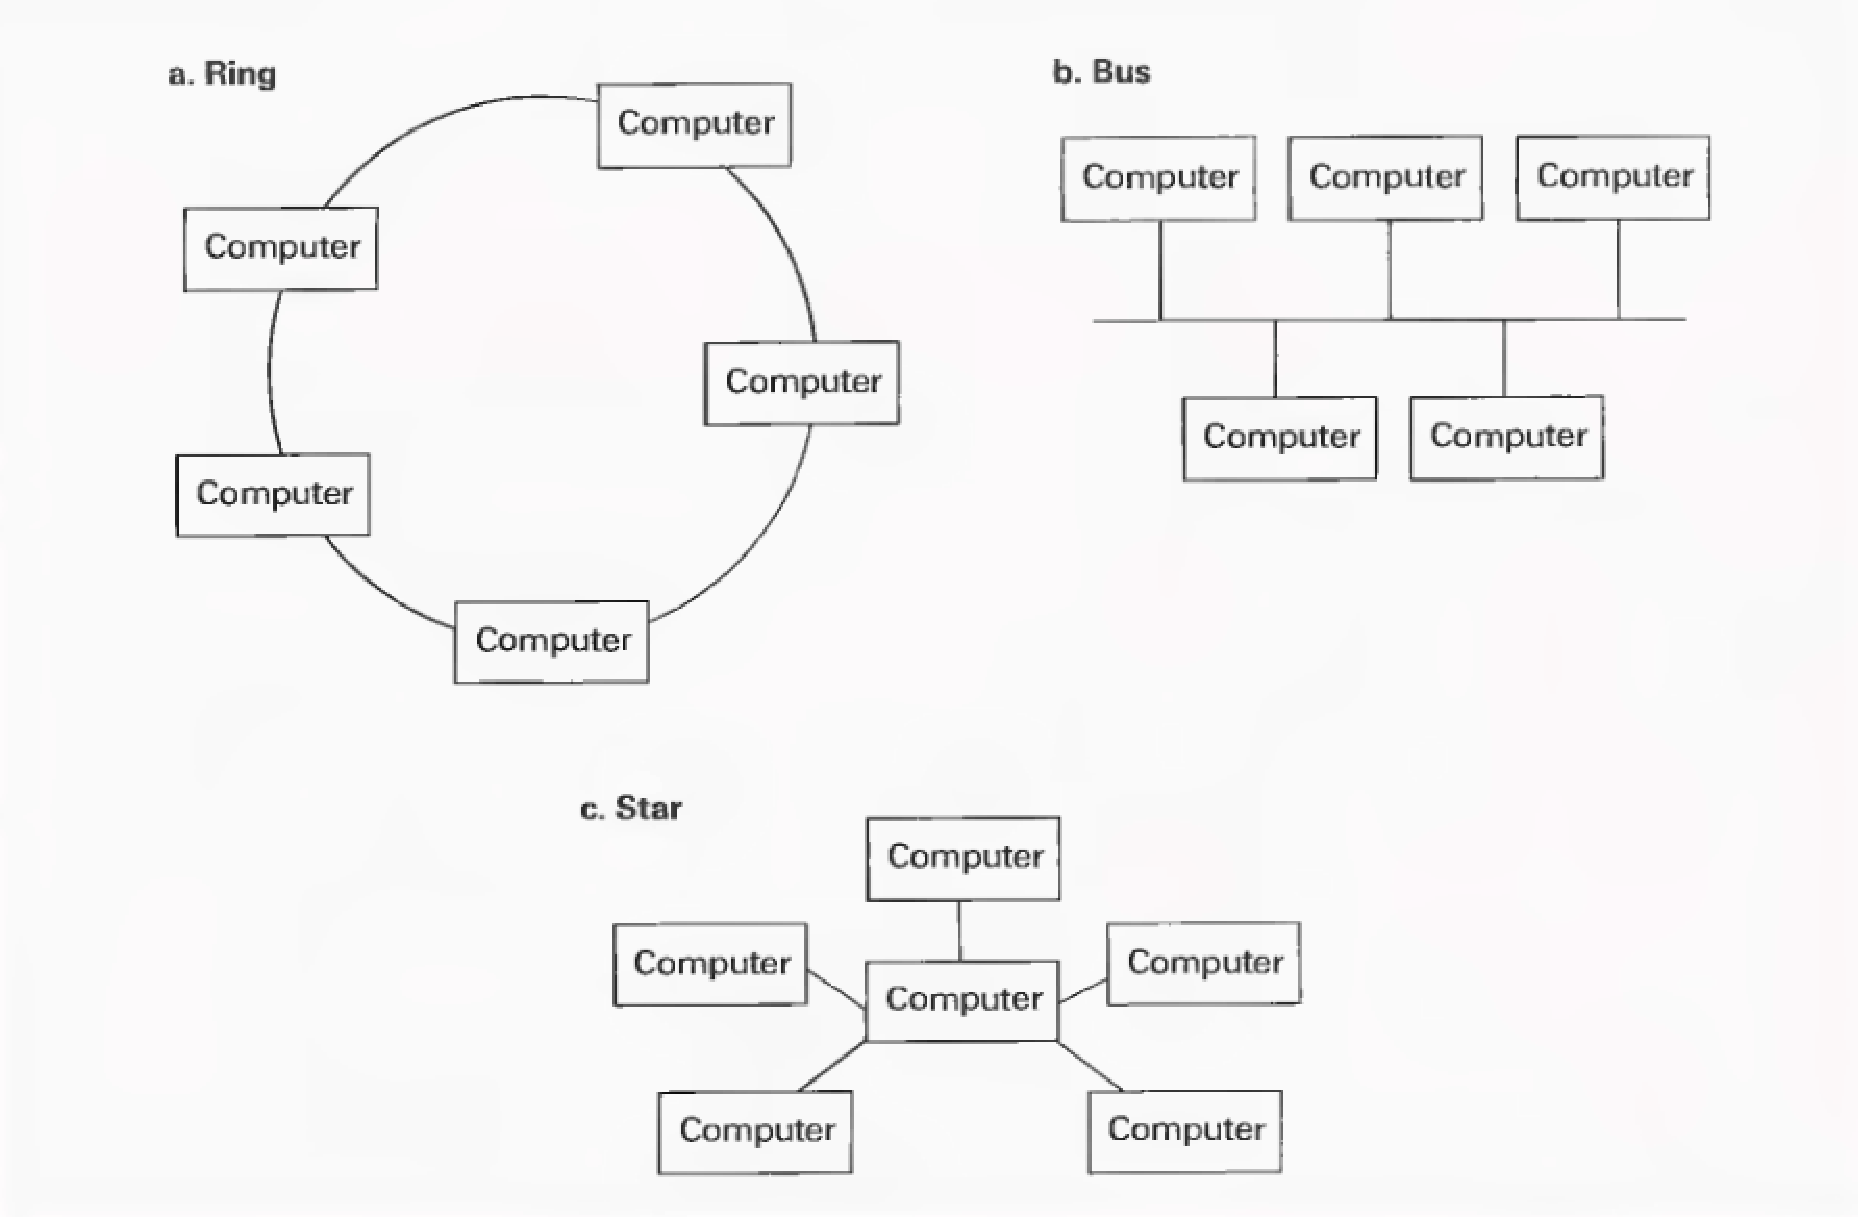
\includegraphics{ch5/fig41.pdf}}
\caption{Các hình trạng mạng}
  \label{fig:fig4.1}
\end{figure}

Còn một cách phân loại mạng khác đó là dựa trên hình trạng của mạng. Hình trạng mạng
là mô hình xác định cách để các thiết bị trong mạng kết nối với nhau. Hình~\ref{fig:fig4.1} giới
thiệu ba hình trạng mạng phổ biến:
\begin{inparaenum}[(1)]
\item Mạng vòng tròn (Ring), trong đó các thiết bị được kết nối với nhau
  theo hình tròn;
\item Mạng hình tuyến (Bus), trong đó tất cả các thiết bị được kết nối với nhau thông qua
  một đường truyền tải gọi là trục chính (Bus); và
\item Mạng hình sao, trong đó một thiết bị phục vụ như là một điểm trung tâm nơi mà các
  thiết bị khác được kết nối tới nó.
\end{inparaenum}

Trong những mô hình trên, mạng hình sao được sử dụng phổ biến nhất. Mạng này đã
phát triển từ mô hình trung tâm máy tính lớn phục vụ cho nhiều người sử dụng. Thể hiện rõ nhất là trường hợp những người dùng sử dụng các thiết bị đầu cuối kết nối vào các máy tính nhỏ. Ngày nay, mô hình mạng hình tuyến (bus) cũng
được sử dụng rộng rãi dưới hình thức mạng chuẩn là \textbf{Ethernet}, một
trong những mô hình mạng khá phổ biến.

Cần chú ý rằng hình trạng của mạng có thể không  thể hiện rõ qua mô hình vật
lý của nó. Ví dụ, một mạng hình tuyến (bus) không nhất thiết phải được triển khai
dưới một đường trục dài nơi mà các máy tính được kết nối thông qua các liên kết ngắn như
đã mô tả trong Hình~\ref{fig:fig4.1}. Thay vào đó, thông thường người ta dựng một mạng
hình tuyến bằng cách chạy các liên kết từ chính mỗi máy tính tới một vùng trung tâm, nơi
mà chúng được kết nối với nhau thông qua một thiết bị gọi là \textbf{hub}. Thiết bị hub
này nhỏ hơn bất kỳ một trục ngắn nào. Nó thực hiện tiếp sóng bất kỳ tín hiệu nào nó nhận
được (thông qua một vài bộ khuếch đại tín hiệu) và truyền tới tất cả các máy tính kết nối
với nó thông qua các cổng. Kết quả là một mạng trông như mạng hình sao lại được hoạt động
dưới hình thức là một mạng hình tuyến. Sự khác nhau ở đây là thiết bị trung tâm trong mô
hình mạng hình sao là một máy tính (thường là một thiết bị với nhiều khả năng hơn tại các
điểm nút của hình sao); nó  nhận và xử lý các thông điệp từ các máy tính khác. Ngược lại, thiết
bị trung tâm trong mô hình mạng hình tuyến là một hub; nó  chỉ đơn thuần cung cấp một kênh truyền
thông tin cho các máy tính.

Một quan điểm khác cũng cần phải chú ý là các kết nối giữa các thiết bị trong hệ thống
mạng không nhất thiết phải là các thiết bị vật lý. Hệ thống mạng không dây, sử dụng công
nghệ truyền phát qua sóng radio, cũng dần được sử dụng phổ biến. Đặc biệt, thiết bị hub
trong rất nhiều mô hình mạng hình tuyến ngày nay thực chất là một trạm tiếp và phát sóng
radio.

\subsection*{Các giao thức}
Để cho một hệ thống mạng hoạt động tin cậy, việc thiết lập những quy tắc nhờ
đó các hoạt động của mạng được kiểm soát là rất quan trọng. Những quy tắc này được gọi là
các \textbf{giao thức}. Thông qua việc phát triển và kế thừa các chuẩn giao thức, các nhà
cung cấp có thể xây dựng những sản phẩm cho các ứng dụng mạng tương thích với những sản
phẩm của nhà cung cấp khác. Việc phát triển các chuẩn giao thức là quá trình không
thể thiếu trong sự phát triển các công nghệ mạng.


Khi giới thiệu về khái niệm giao thức, ta hãy xem xét vấn đề  phối hợp truyền thông điệp giữa các máy tính trong một mạng. Nếu không có các quy tắc  quản lý quá
trình truyền  này, các máy tính có thể yêu cầu truyền thông điệp vào cùng một
thời điểm hoặc cũng có thể bị lỗi khi tiếp nhận các thông điệp khi hỗ trợ đó được yêu cầu.


\begin{figure}[tbh] 
\centering
    \scalebox{0.45}{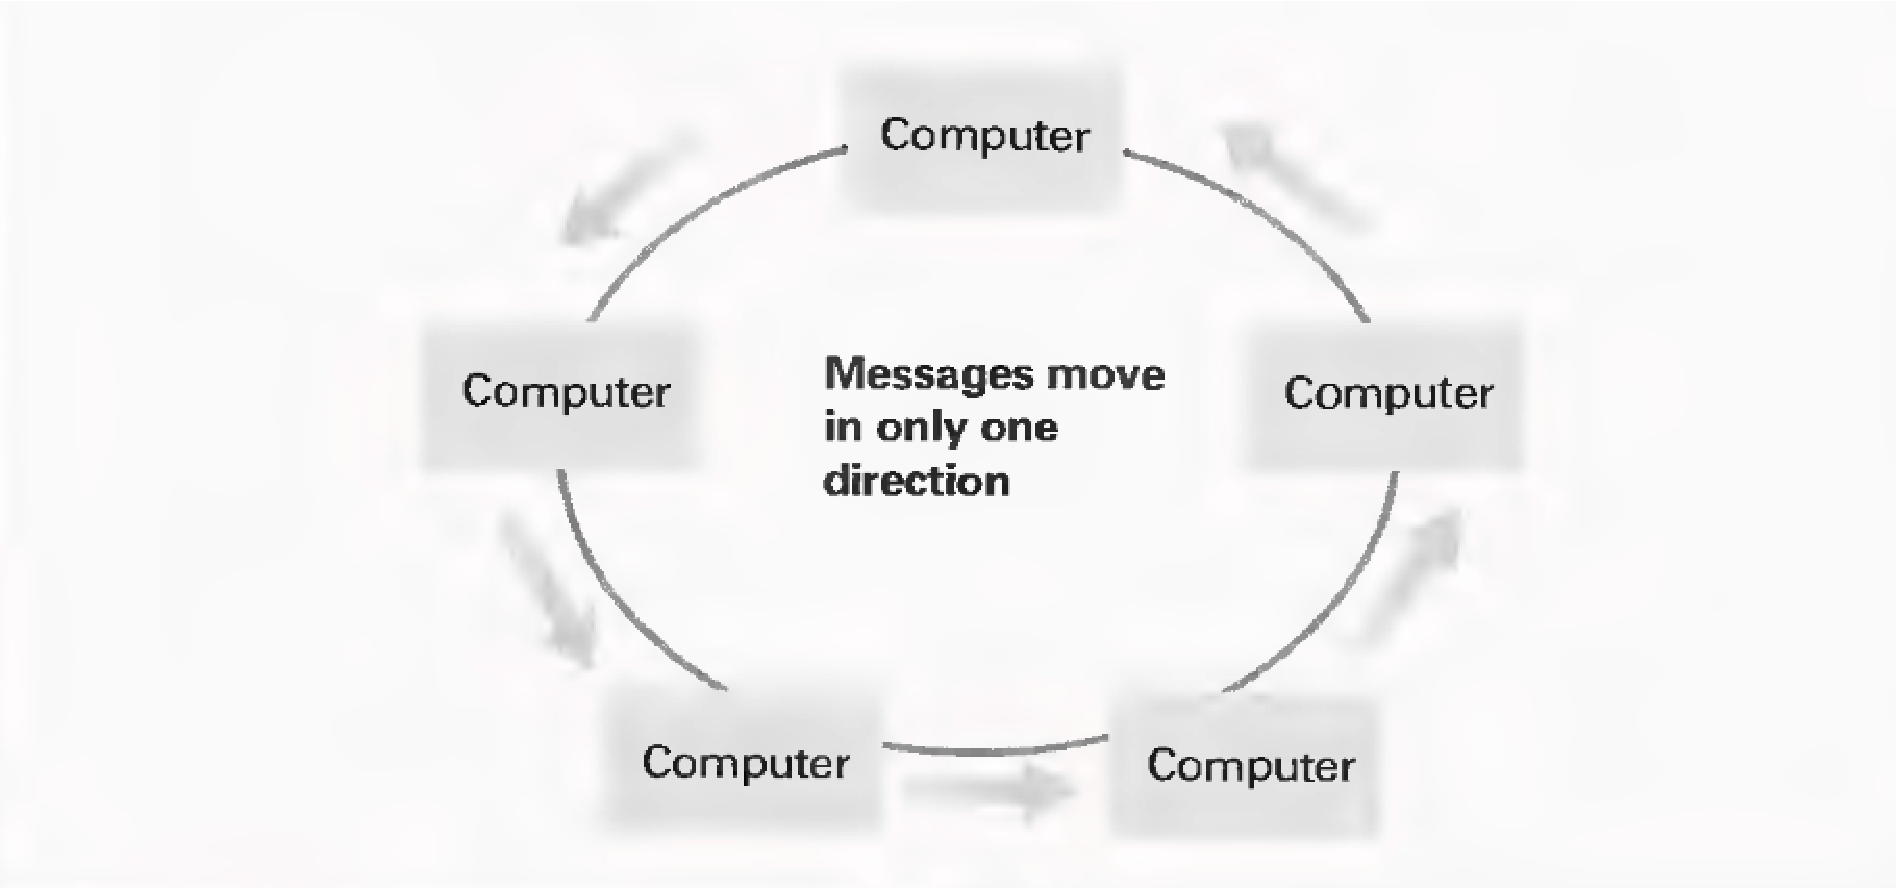
\includegraphics{ch5/fig42.pdf}}
    \caption{Truyền thông trong mạng vòng tròn}
  \label{fig:fig4.2}
\end{figure}

Một cách tiếp cận để có thể giải quyết được vấn đề này là giao thức \textbf{thẻ bài} trong
mạng vòng, được phát triển bởi IBM từ  những năm 1970 và tiếp tục trở nên phổ biến
trong các hệ thống mạng dựa trên nền tảng mô hình mạng vòng. Với giao thức này, tất
cả các thiết bị trong mạng truyền tải thông điệp theo một hướng chung duy nhất
(Hình~\ref{fig:fig4.2}), nghĩa là tất cả các thông điệp đó được gửi qua mạng di chuyển
vòng tròn theo cùng một hướng bằng cách chuyển tiếp từ máy tính này tới máy tính khác. Khi
một thông điệp được truyền tới đích của nó, máy tính đích giữ lại một bản sao và chuyển
tiếp một bản sao của thông điệp đó sang máy tính tiếp theo theo hình tròn. Khi bản sao
được chuyển tiếp về tới máy tính ban đầu, máy tính đó nhận thấy rằng thông điệp này đã
truyền được tới đích cần thiết, nó sẽ loại bỏ thông điệp ra khỏi vòng tròn. Tất nhiên, hệ
thống này còn phụ thuộc vào sự hợp tác của các liên máy tính. Nếu một máy tính yêu cầu
truyền phát liên tục các thông điệp từ chính nó thay vì chuyển tiếp các thông điệp sang
máy tính khác thì không có quá trình truyền tải nào được hoàn thành.


Để giải quyết vấn đề này, một xâu bít duy nhất, gọi là thẻ bài, được sử dụng trong quá
trình truyền tải theo vòng tròn. Quyền sở hữu của thẻ bài này được trao cho máy tính
nguồn, nơi bắt đầu truyền phát thông điệp; nếu không có thẻ bài, một máy tính chỉ được
phép chuyển tiếp thông điệp mà nó nhận được. Thông thường, mỗi máy tính đơn thuần chỉ tiếp
nhận và chuyển tiếp thẻ bài theo đúng cách mà nó chuyển tiếp thông điệp. Tuy nhiên, nếu
máy tính nhận được thẻ bài có thông điệp của chính nó đưa lên mạng, nó sẽ truyền một thông
điệp trong khi giữ lại thẻ bài. Khi thông điệp này hoàn tất quá trình truyền tải qua một
vòng tròn, máy tính chuyển tiếp thẻ bài cho máy tính tiếp theo trong vòng tròn. Như vậy,
khi máy tính tiếp theo nhận được thẻ bài, nó có thể chuyển tiếp thẻ bài ngay lập tức hoặc
truyền phát một thông điệp mới của mình trước khi chuyển tiếp thẻ bài cho máy tính tiếp
theo. Theo cách thức này, mỗi máy tính trong mạng đều có cơ hội như nhau để có thể gửi
thông điệp của nó cũng như thẻ bài đi xung quanh vòng tròn.


\begin{figure}[tbh]
\centering
    \scalebox{0.4}{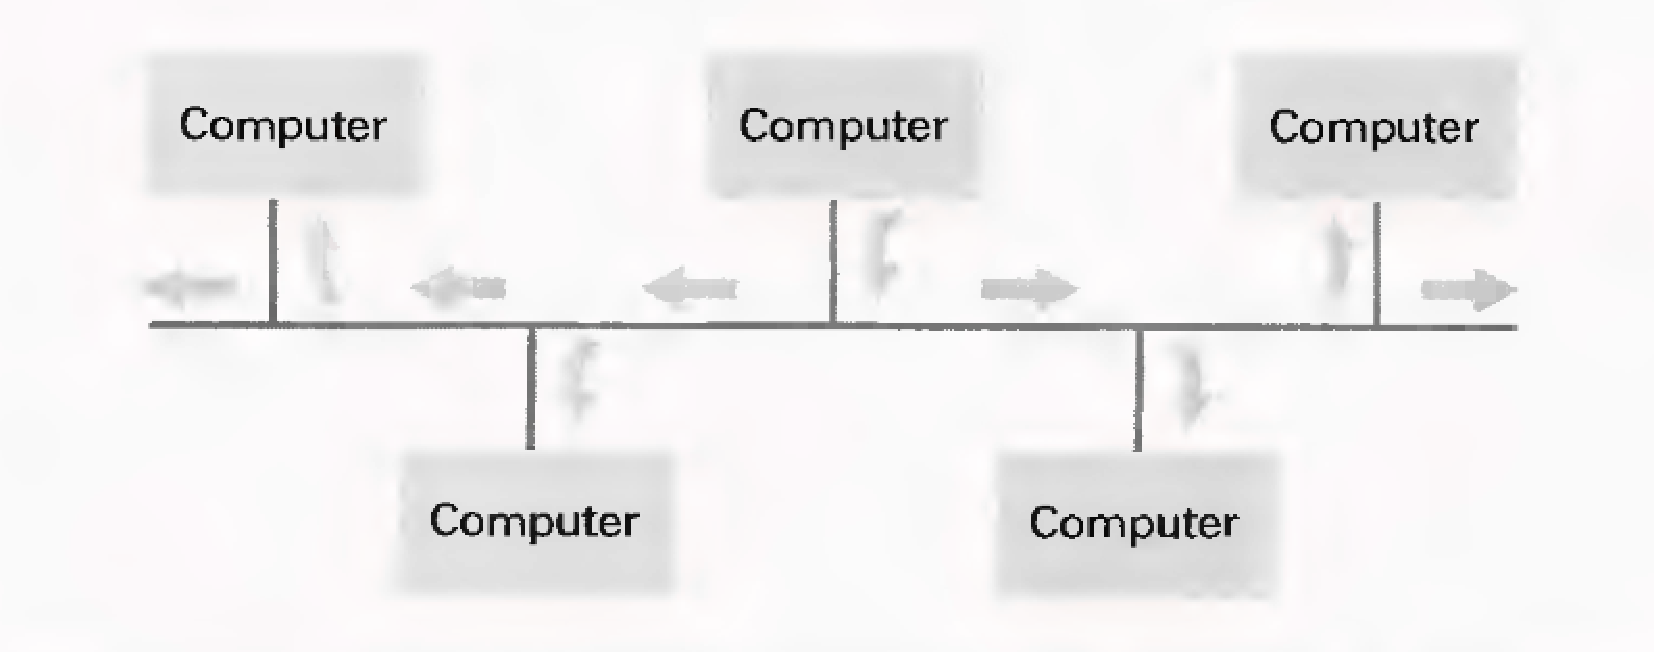
\includegraphics{ch5/fig43.pdf}}
    \caption{Truyền thông trong mạng hình tuyến}
  \label{fig:fig4.3}
\end{figure}

Một giao thức khác cũng được sử dụng trong công nghệ mạng hình tuyến cho việc phối hợp
truyền tải các thông điệp, đó là giao thức dựa trên tập các giao thức Ethernet. Trong hệ
thống mạng Ethernet, quyền truyền tải thông điệp được điều khiển bởi giao thức \textbf{Đa
  truy nhập có thăm dò và tách đụng độ} (Carrier Sense, Multiple Access with Collision
Detection--CSMA/CD). Giao thức này yêu cầu mỗi thông điệp phải được quảng bá cho tất cả
các máy tính trong trục chính (Hình~\ref{fig:fig4.3}). Mỗi máy tính sẽ theo dõi tất cả các
thông điệp những chỉ giữ lại những thông điệp nào được gửi tới chính nó thông qua địa
chỉ. Để truyền phát một thông điệp, một máy tính đợi cho đến khi đường trục chính rỗi, và
tại thời điểm này nó sẽ bắt đầu truyền phát tín hiệu trong khi tiếp tục theo dõi đường
trục chính. Nếu một máy tính khác cũng bắt đầu truyền tín hiệu, cả hai máy tính sẽ phát
hiện ra sự xung đột và sẽ tạm dừng trong một khoảng thời gian ngẫu nhiên trước khi truyền
tín hiệu lại. Một nhóm nhỏ người có nhu cầu đàm luận với nhau có thể sử dụng một hệ thống
tương đương như vậy. Nếu hai người cùng bắt đầu nói tại một thời điểm, cả hai sẽ dừng
lại. Một trong hai người có thể sẽ tiếp tục với một chuỗi câu như ``Xin lỗi, anh định nói
gì vậy?'', ``Không, không. Anh nói trước đi'', trong khi với giao thức CSMA/CD, mỗi máy
tính đơn thuần chỉ là thử truyền phát tín hiệu lại.


\subsection*{Kết hợp các hệ thống mạng}

Đôi khi cần phải kết nối các hệ thống mạng đã tồn tại thành một hệ thống truyền thông mở
rộng. Điều này có thể được thực hiện bằng việc kết nối các mạng thành một phiên bản lớn
hơn nhưng vẫn cùng ``kiểu'' như hệ thống cũ. Ví dụ, trong trường hợp những hệ thống mạng
hình tuyến dựa trên các giao thức mạng Ethernet, thông thường có thể kết nối các trục
chính thành một trục đơn lớn hơn. Việc này được thực hiện với điều kiện sử dụng các thiết
bị khác nhau được biết đến như\textbf{ bộ lặp tín hiệu} (repeater), \textbf{cầu nối}
(bridge), và \textbf{bộ chuyển mạch} (switch), đó là những sự khác biệt không dễ phát hiện
ra nhằm phục vụ cho việc mở rộng hệ thống mạng. Đơn giản nhất trong số đó là bộ lặp tín
hiệu, thiết bị dùng để kết nối trục chính của hai mạng hình tuyến lại với nhau thành một
trục dài hơn (Hình~\ref{fig:fig4.4}). Bộ khuếch đại (bộ lặp tín hiệu) đơn giản chỉ truyền
các tín hiệu về phía sau hay trước giữa hai tuyến gốc ban đầu (thông thường sử dụng với
một vài bộ khuếch đại tín hiệu) mà không cần biết ý nghĩa của những tín hiệu đó là gì.

\begin{figure}[tb] 
  \centering \scalebox{0.45}{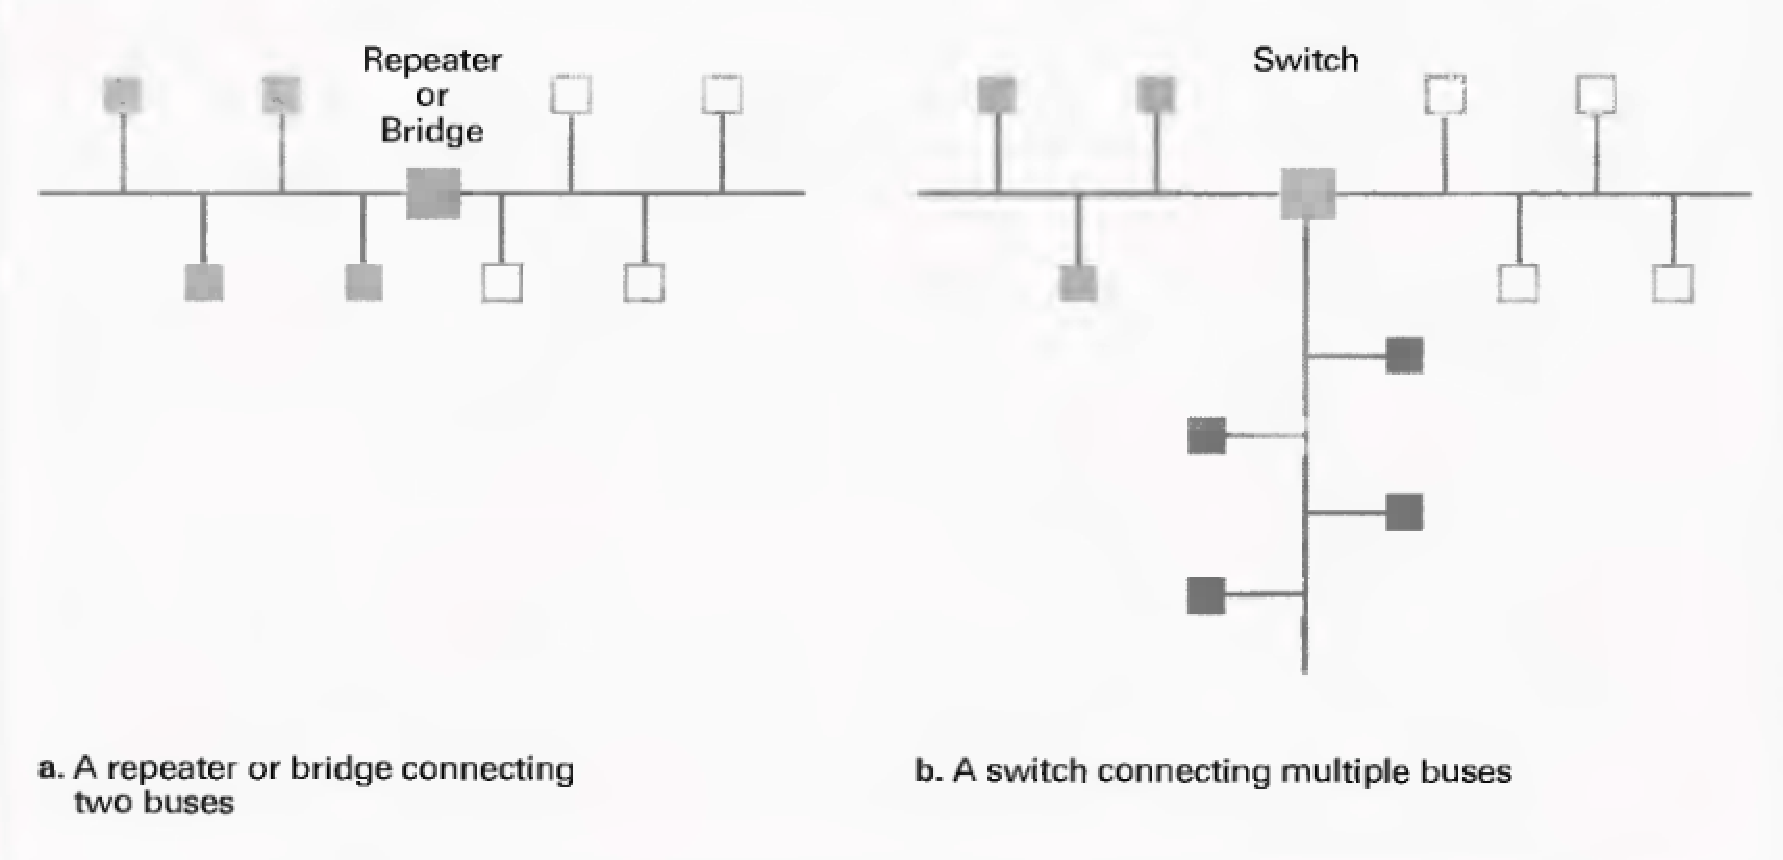
\includegraphics{ch5/fig44.pdf}}
  \caption{Xây dựng một mạng hình tuyến lớn từ những mạng nhỏ hơn}
  \label{fig:fig4.4}
\end{figure}

\textbf{Cầu nối} là một thiết bị tương đương, nhưng phức tạp hơn so với bộ lặp tín
hiệu. Cũng như bộ lặp tín hiệu, cầu nối kết nối hai mạng hình tuyến với nhau, nhưng nó
không nhất thiết phải chuyển tiếp tất cả các thông điệp từ tuyến này sang tuyến kia. Thay
vào đó, nó sẽ xem địa chỉ đích đi kèm với thông điệp và chuyển tiếp thông điệp qua kết nối
chỉ khi thông điệp đó đã được chỉ định trước là sẽ được gửi tới một máy tính ở phía bên
kia của kết nối. Do đó, hai thiết bị nằm ở trên cùng một phía của cầu nối có thể trao đổi
thông điệp mà không gây phiền phức cho sự truyền thông ở phía bên kia của cầu. Cầu nối
thường làm việc có hiệu quả hơn so với bộ lặp tín hiệu.

\textbf{Bộ chuyển mạch} về bản chất là một cầu nối có nhiều cổng kết nối, cho phép nó kết
nối tới nhiều hơn hai tuyến. Do đó, bộ chuyển mạch tạo ra một mạng bao gồm một vài tuyến
được mở rộng từ bộ chuyển mạch như những chiếc nan hoa của bánh xe
(Hình~\ref{fig:fig4.4}b). Cũng giống như cầu nối, bộ chuyển mạch sẽ xem xét địa chỉ đích
của tất cả các thông điệp và chỉ chuyển tiếp những thông điệp nào đã được chỉ định trước
sang các tuyến khác. Hơn nữa, mỗi thông điệp được chuyển tiếp chỉ được chuyển tới các
tuyến tương ứng của địa chỉ đích, chính vì vậy mà nó có thể giảm thiểu được giao thông
trên mỗi tuyến.

Cần phải chú ý rằng khi các mạng được kết nối với những thiết bị như bộ lặp tín hiệu, cầu
nối hay thiết bị chuyển mạch, kết quả là một mạng đơn lớn hơn được tạo ra. Mỗi máy tính
tiếp tục truyền tải thông qua hệ thống theo cách thức cũ (sử dụng cùng một giao thức mạng)
nếu hệ thống được xây dựng ban đầu như là một mạng đơn lớn. Điều đó có nghĩa là, các máy
tính cá nhân trong hệ thống không cần biết đến sự tồn tại của các bộ lặp tín hiệu, các cầu
nối, hay các thiết bị chuyển mạch.

Tuy nhiên, các hệ thống mạng được kết nối đôi khi cũng có những đặc tính không tương thích
nhau. Ví dụ, những đặc tính của mạng vòng tròn sử dụng giao thức thẻ bài vòng tròn
không tương thích với mạng Ethernet hình tuyến sử dụng CSMA/CD. Trong những trường hợp
này, các hệ thống mạng cần phải được kết nối theo một cách thức dùng để tạo ra hệ thống
mạng của các mạng, được biết đến như là hệ thống \textbf{liên mạng} (internet), trong đó
những mạng gốc ban đầu duy trì những tính chất riêng của chúng và tiếp tục vận hành như là
những hệ thống độc lập. (Chú ý rằng \textit{liên mạng (internet)} khác với mạng
\textit{Internet}. Mạng Internet, với chữ cái I được viết hoa, được nói đến như một hệ
thống liên mạng đặc biệt, có phạm vi rộng lớn mà ta sẽ nghiên cứu trong một phần khác của
chương này. Có rất nhiều ví dụ về những hệ thống liên mạng. Quả thực, hệ thống truyền
thông qua điện thoại cổ điển đã được sử dụng khá tốt trong các hệ thống liên mạng phạm vi
rộng trước khi mà mạng Internet được phổ biến.)


\begin{figure}[tb] 
  \centering \scalebox{0.45}{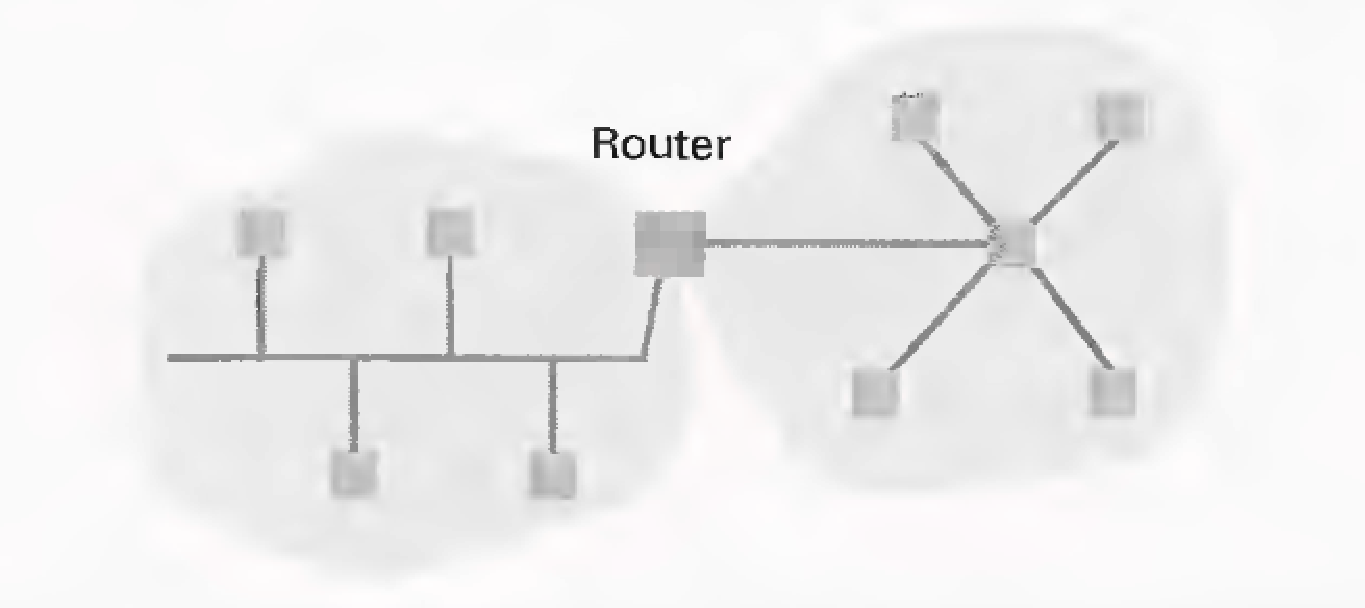
\includegraphics{ch5/fig45.pdf}}
  \caption{Bộ dẫn đường kết nối một mạng hình tuyến với một mạng hình sao tạo thành một hệ
    thống liên mạng}
  \label{fig:fig4.5}
\end{figure}

Sự kết nối giữa hai hệ thống mạng tạo thành một hệ thống liên mạng được thực hiện bởi một
thiết bị gọi là \textbf{bộ dẫn đường} (Router). Một bộ dẫn đường là một máy tính thuộc về
cả hai hệ thống mạng ở hai phía của nó với nhiệm vụ là chuyển tiếp các thông điệp từ mạng
này sang mạng kia (Hình~\ref{fig:fig4.5}). Chú ý rằng nhiệm vụ của bộ dẫn đường đặc biệt
to tát hơn nhiều so với các thiết bị như bộ lặp tín hiệu, cầu nối hay thiết bị chuyển mạch
bởi vì một bộ dẫn đường cần phải thực hiện chuyển đổi giữa các đặc tính riêng biệt của hai
mạng gốc ban đầu. Ví dụ, khi truyền phát một thông điệp từ một mạng sử dụng giao thức thẻ
bài vòng tròn tới một mạng sử dụng giao thức CSMA/CD, bộ dẫn đường phải nhận thông điệp sử
dụng một giao thức sau đó lại sử dụng một giao thức khác để truyền thông điệp đó tới mạng
kia.


Ta sẽ xem xét một ví dụ khác sẽ mô tả sự phức tạp khi thực hiện việc dẫn đường của
Router. Đó là vấn đề khi hai mạng kết nối với nhau lại sử dụng hai hệ thống địa chỉ khác
nhau để xác định các máy tính trong mạng. Khi một máy tính trong một mạng muốn gửi một
thông điệp tới một máy tính ở mạng bên kia, nó không thể xác định được máy tính đích theo
cách thức thông thường mà nó vẫn thường thực hiện.

\begin{figure}[t]
  \begin{quotation}
    \noindent
    \textbf{Mạng Enthernet} \vspace{0.3cm}
    \\
    Mạng Ethernet là một tập các chuẩn được triển khai trong một mạng LAN với mô hình mạng
    hình tuyến. Tên gọi của nó được bắt nguồn từ thiết kế mạng Ethernet ban đầu trong đó
    các thiết bị được kết nối với nhau qua cáp đồng trục. Khởi đầu mạng Ethernet được phát
    triển vào những năm 1970 và ngày nay được chuẩn hóa bởi IEEE là một phần của họ chuẩn
    IEEE 802, mạng Ethernet có hầu hết các cách thức chung của một mạng các máy tính. Việc
    cài đặt các card điều khiển mạng của các máy tính cá nhân trong mạng Ethernet có thể
    thực hiện được và khá dễ dàng.

    Ngày nay trên thực tế có một vài phiên bản của mạng Ethernet với những công nghệ tiên
    tiến hơn và tốc độ truyền tải thông tin cũng cao hơn. Tuy nhiên, tất cả những phiên
    bản mới đó vẫn có đủ các đặc tính chung của họ mạng Ethernet. Mỗi một phiên bản trong
    số đó là một khuôn thức mà trong đó dữ liệu được đóng gói trước khi truyền đi, sử dụng
    mã hóa Manchester (một phương pháp mà trong đó đại diện là các bít 0 và 1, với một bít
    0 sẽ đại diện cho một tín hiệu giảm dần và bít 1 đại diện cho một tín hiệu tăng dần)
    để truyền tải thực sự các bít dữ liệu, và sử dụng giao thức CSMA/CD để điều khiển
    quyền truyền phát.
  \end{quotation}
\end{figure}

Trong những trường hợp như vậy, một hệ thống địa chỉ với phạm vi liên mạng được thiết
lập. Kết quả là mỗi thiết bị trong một hệ thống liên mạng có hai địa chỉ: một địa chỉ của
chính mạng gốc ban đầu của nó và một địa chỉ liên mạng mới. Để gửi một thông điệp từ một
máy tính thuộc một trong những mạng gốc tới một máy tính trong mạng khác--máy tính có địa chỉ
liên mạng của gói tin gốc ban đầu, nó sẽ sử dụng hệ thống địa chỉ gốc của mạng cục bộ để
gửi gói tin tới bộ dẫn đường. Bộ dẫn đường sau đó sẽ xem xét bên trong của gói tin nhận
được, thực hiện tìm địa chỉ liên mạng đích sau cùng của thông điệp, dịch địa chỉ đó thành
địa chỉ có định dạng thích hợp với mạng kia, sau đó chuyển tiếp thông điệp tới đích của
nó. Nói một cách ngắn gọn, các thông điệp trong mỗi một mạng gốc tiếp tục được truyền theo
cách thức của hệ thống địa chỉ gốc của mỗi mạng, và bộ dẫn đường được phân công nhiệm vụ
là chuyển đổi giữa các hệ thống.

\subsection*{Truyền thông liên tiến trình}
Các tiến trình thực thi trên các máy tính khác nhau trong một mạng
máy tính (hay thậm chí trên cùng một máy  theo cách thức chia sẻ thời gian)
thường phải liên lạc với các tiến trình khác  để thực hiện những nhiệm vụ đã được xác định. Việc liên lạc này được gọi là sự \textbf{truyền thông liên tiến trình}.

Một trong những phương thức phổ biến trong truyền thông liên tiến trình là mô hình
\textbf{khách/chủ} (client/server). Mô hình này xác định  vai trò của các tiến
trình trên máy trạm, nơi mà sẽ phát sinh các yêu cầu tới các tiến trình khác trên máy chủ, và các tiến trính trên máy chủ  
nơi sẽ thực hiện các yêu cầu của máy trạm.

Một ứng dụng sơ khai trong mô hình khách/chủ đã xuất hiện trên những mạng liên kết tất cả
máy tính trong một nhóm các văn phòng. Trong tình huống như vậy, một máy in đơn lẻ, chất
lượng cao được kết nối vào mạng nơi mà tất cả các máy tính trong đó có thể sử dụng được
máy in đó. Với trường hợp này máy in đã đóng vai trò của một máy chủ (thường được gọi là
\textbf{máy chủ in} (printer server), và các máy tính khác được lập trình để đóng vai của
các máy trạm sẽ gửi các yêu cầu in ấn tới máy chủ in.

Một ứng dụng khác của mô hình khách/chủ cũng sớm được đưa vào sử dụng nhằm giảm chi phí
lưu trữ bằng cách loại bỏ những nhu cầu về các bản sao trùng lặp của những mẫu tin. Ở đây,
một máy tính trong mạng được trang bị một hệ thống lưu trữ thứ cấp có khả năng cao (thường
sử dụng một đĩa từ) mà trên đó chứa toàn bộ các thông tin dữ liệu của một đơn vị. Các máy
tính khác trên mạng có thể yêu cầu truy cập tới các thông tin dữ liệu mà chúng cần. Khi
đó, máy tính chứa thông tin dữ liệu đóng vai trò là một máy chủ (gọi là \textbf{máy chủ
  file}--file server), và các máy tính khác đóng vai trò là các máy trạm sẽ gửi các yêu
cầu truy cập với những file dữ liệu được lưu trữ trên máy chủ file.

\begin{figure}[tb] 
  \centering \scalebox{0.4}{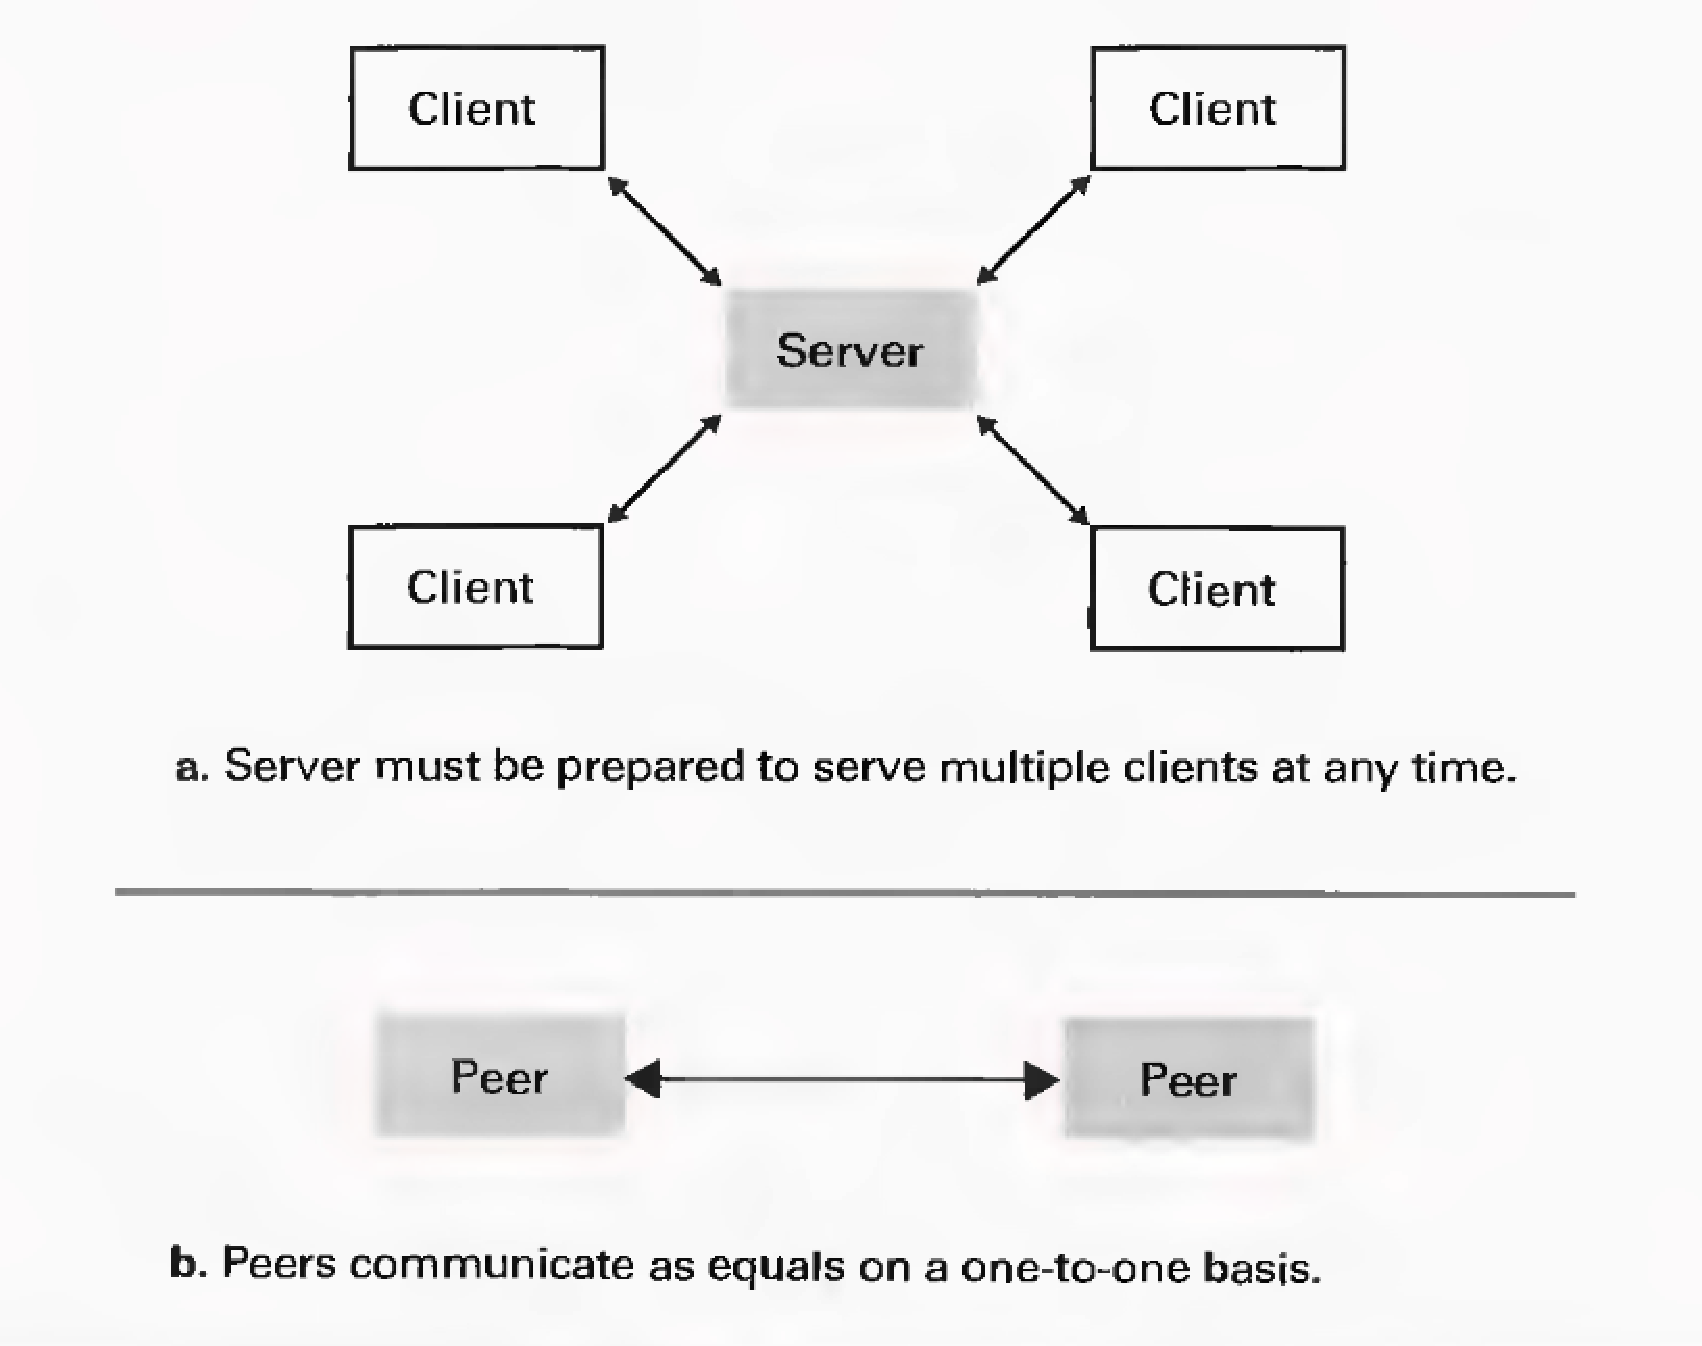
\includegraphics{ch5/fig46.pdf}}
  \caption{Mô hình client/server so sánh với mô hình peer-to-peer}
  \label{fig:fig4.6}
\end{figure}

Ngày nay, mô hình khách/chủ được sử dụng rộng rãi trong các ứng dụng mạng, ta sẽ xem xét ở
phần sau trong chương này. Tuy nhiên, không chỉ mô hình khách/chủ mới hoạt động theo cách
thức như một sự truyền thông liên tiến trình. Một mô hình khác với tên gọi
\textbf{peer-to-peer} (thường được viết tắt là P2P), có những tính chất trái ngược hoàn
toàn với mô hình khách/chủ. Trong khi mô hình khách/chủ bao gồm một tiến trình (trên máy
chủ) thực hiện liên lạc với nhiều tiến trình khác (tại các máy trạm) thì mô hình
peer-to-peer lại bao gồm hai tiến trình trao đổi ngang hàng với nhau
(Hình~\ref{fig:fig4.6}). Ngoài ra, một máy chủ phải chạy liên tục nhằm phục vụ cho các máy
trạm của nó tại bất kỳ thời điểm nào, ngược lại mô hình peer-to-peer với hai tiến trình có
thể thực hiện theo cách thức tạm thời. Ví dụ, các ứng dụng trong mô hình peer-to-peer bao
gồm việc gửi tức thì các thông điệp mà hai người thực hiện đối thoại với nhau qua Internet
cũng như những tình huống như hai người chơi những trò chơi như cờ vua hay cờ đam (một
loại trò chơi gồm 24 quân cờ cho 2 người chơi).


Mô hình peer-to-peer cũng hoạt động theo cách thức chia sẻ file như các bản nhạc hay những
bộ phim qua Internet (đôi khi đi kèm là vấn đề về bản quyền). Trong trường hợp này, những
cá nhân cần tìm kiếm những khoản mục phổ biến có thể quảng bá mong muốn của họ lên
Internet và liên hệ được với những ai sở hữu những khoản mục đó. Sau đó, những khoản mục
này được truyền tải giữa hai phía sử dụng mô hình peer-to-peer. Điều này trái ngược hoàn
toàn với cách tiếp cận của mô hình khách/chủ qua việc thiết lập một ``trung tâm phân
phối'' (máy chủ file) cho các máy trạm tải các bản nhạc (hay ít nhất là tìm thấy các nguồn
của những khoản mục đó). Tuy nhiên, máy chủ trung tâm, đã chứng thực được là một điểm
trung tâm mà tại đó ngành công nghiệp âm nhạc có thể được tuân thủ theo đúng luật bản
quyền, dẫn tới kết quả cuối cùng là sự dỡ bỏ các trung tâm phân phối âm nhạc. Ngược lại,
sự thiếu vắng các trung tâm điều hành như vậy trong mô hình peer-to-peer sẽ khiến nỗ lực
làm cho luật bản quyền có hiệu lực trở nên khó khăn.

Thông thường bạn có thể đọc và nghe về \textit{mạng peer-to-peer}, ví dụ như việc sử dụng
sai những thuật ngữ có thể mắc phải khi những ngôn từ kỹ thuật được thông qua bởi một cộng
đồng phi kỹ thuật. Mạng \textit{peer-to-peer} được biết đến như một hệ thống mà trong đó,
hai tiến trình trao đổi với nhau qua mạng (hoặc liên mạng). Nó không phải là một thuộc
tính của mạng (hay liên mạng). Một tiến trình có thể sử dụng mô hình peer-to-peer để trao
đổi với tiến trình khác thông qua cùng một hệ thống mạng. Vì vậy cần phải nói một cách
chính xác là truyền thông theo cách thức của mô hình peer-to-peer chứ không phải là truyền
thông qua một mạng peer-to-peer.

\subsection*{Các hệ thống phân tán}
Với sự thành công của công nghệ mạng, sự tương tác giữa những máy tính qua các hệ thống
mạng trở nên phổ biến và được thể hiện ở nhiều khía cạnh. Nhiều hệ thống phần mềm hiện
đại, như các hệ thống tìm kiếm hay phục hồi thông tin toàn cầu, các hệ thống kiểm toán có
phạm vi toàn công ty, các trò chơi máy tính, và thậm chí các phần mềm điều khiển chính hệ
thống cơ sở hạ tầng của mạng được thiết kế như là những \textbf{hệ thống phân tán}. Điều
đó có nghĩa là chúng gồm có những đơn vị phần mềm được thực thi dưới dạng các tiến trình trên
các máy tính khác nhau. Ta có thể hình dùng những tiến trình này như là những vị khách cư
trú tại các máy tính khác nhau mà qua đó các máy tính trong một mạng sẽ được gọi là các
\textbf{máy chủ} (host). Điều đó có nghĩa rằng host là một máy tính mà các tiến trình
trú ngụ trên đó theo một hay nhiều ngữ cảnh.

Các hệ thống phân tán đầu tiên được phát triển độc lập từ những hệ thống hỗn tạp. Nhưng
ngày nay, việc nghiên cứu một cách cẩn thận đã cho thấy một cơ sở hạ tầng phổ biến vận
hành trong suốt toàn bộ những hệ thống này, bao gồm cả những thứ như các hệ thống truyền
thông và bảo mật. Đổi lại, kết quả của sự cố gắng đã tạo ra các hệ thống mà có thể cung
cấp cơ sở hạ tầng cơ bản và chính vì vậy, nó cho phép các ứng dụng phân tán được xây dựng
bởi sự phát triển phần hệ thống duy nhất đối với ứng dụng đó.

Một kết quả của nhận định trên là hệ thống đặc tả về giao diện lập trình JavaBeans (được
phát triển bởi Sun Microsystems). Hệ thống này là một môi trường phát triển trợ giúp việc
xây dựng các hệ thống phần mềm phân tán mới. Sử dụng JavaBeans, một hệ thống phân tán được
xây dựng từ những đơn vị được gọi là các bean được tự động thừa kế những đặc tính cơ sở hạ
tầng của hệ thống cha. Do đó, chỉ có những thành phần ứng dụng phụ thuộc duy nhất của một
hệ thống mới mới được phát triển. Một cách tiếp cận khác là môi trường phát triển phần mềm
với tên gọi .NET Framework (được phát triển bởi Microsoft). Với thuật ngữ .NET, các thành
phần của hệ thống phân tán được gọi là các assembly. Mặt khác, bằng việc phát triển các
đơn vị này trong môi trường .NET, chỉ những nét đặc trưng duy nhất đối với một ứng dụng
phổ biến là cần phải được xây dựng dựa trên nền tảng cơ sở hạ tầng có sẵn. Cả hai môi
trường JavaBeans và .NET Framework đều rất đơn giản trong việc phát triển các hệ thống
phần mềm phân tán mới.

\subsection*{Câu hỏi \& Bài tập}

\begin{enumerate}
\item Thế nào là một hệ thống mạng mở?

\item Tóm tắt những đặc tính khác biệt giữa thiết bị lặp tín hiệu và cầu nối

\item Thiết bị dẫn đường là gì?

\item Mô tả một vài mối quan hệ trong xã hội tuân theo mô hình khách/chủ.

\item Mô tả một vài giao thức được sử dụng trong xã hội.

\end{enumerate}



%%% Local Variables: 
%%% mode: latex
%%% TeX-master: "../tindaicuong"
%%% End: 
